\chapter{Design und Design-Entscheidungen}
%Modul Überblick-bild
Die Betriebssoftware wurde in Module aufgeteilt. Ein Modul kann mehrere Code-Dateien
umfassen. Eine Code-Datei ist aber nur einem Modul zugeordnet.
Es wurde besonderer Wert darauf gelegt, dass Module so wenig wie möglich andere
Module aufrufen, und dies auch nur durch Funktionen, nicht durch die Variablen.
Dieses Prinzip musste allerdings während der Optimierungs- und Testphase
geringfügig modifiziert werden. Entweder wurde der Code dadurch unleserlich, oder
die Relation Preis zu Nutzen je Funktionsaufruf unangemessen hoch.
Als wesentliche Verbesserung wurden vier bis fünf globale Variablen eingeführt, die
sich während der Laufzeit ändern können, und die in unterschiedlichen Modulen direkt
referenziert werden.
Geändert werden diese allerdings nur in sehr wenigen Funktionen, in denen dies
auch explizit dokumentiert wurde. Außerdem wurde in den Coding-Guidelines darauf hingewiesen,
möglichst keine Funktionen zu schreiben, die die globalen Variablen verändern.
Anderenfalls ist dies ausdrücklich hervorzuheben.
Neben diesen maximal fünf globalen Variablen, die das Systemverhalten verändern, gibt es vier
weitere Variablen in zwei verschiedenen Modulen, die jeweils aus einem anderen
Modul gesetzt werden. Dies sind die Trigger-Werte für die Position und
die Zeit. Diese werden nur durch den Drive bzw. den Advanced-Drive-Befehl
gesetzt und während der Motorunterbrechungen nach und nach dekrementiert.
Auf die Module wird in den Unterkapiteln genauer eingegangen.
\section{System}
Das als System bezeichnete Modul beinhaltet die Hauptschleife der Betriebssoftware
und die Initialisierung aller anderen Untermodule. Es benutzt nur wenige Module,
um seine Aufgabe in einem abstrakten Maße zu erfüllen. Während der Hauptschleife, die
in gekürzter Fassung (d.h., ohne Kommentare und Debug-Ausgaben) in Abb. \ref{main_loop} zu sehen ist,
werden nur einige wenige Funktionen aufgerufen. Dadurch werden die wichtigen Module auf dem
aktuellen Stand gehalten. Außerdem wird es ermöglicht, dass Daten zwischen den Modulen fließen können.
\begin{figure}[htb]
 \centering
 \scalebox{0.5}{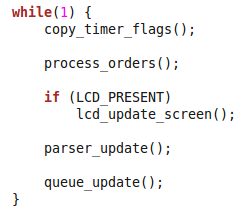
\includegraphics{pictures/main_loop_code.png}}
 \caption{\label{main_loop}Die Hauptschleife}
\end{figure}
\section{Debug}
Eigene Mechanismen zum Debugging sind gerade dann wichtig, wenn man dies nicht mit den
gewohnten Werkzeugen durchführen kann.
Es ist unabdingbar wichtig zu wissen, welche Vorgänge sich in dem kleinen Mikrocontroller
während der Laufzeit abspielen.
Dies ist aber nicht ganz einfach, denn die einzigen Möglichkeiten, die die Platine zur
Kommunikation mit der Außenwelt hat, beschränken sich auf
5 LED, ein 4*20-Zeichen-LCD, eine UART- und eine I2C-Bus-Schnittstelle.
Die LED funktionieren nicht zuverlässig und das LCD ist in seinem Aussagegehalt sehr
begrenzt, weil man nicht viele Informationen auf einem 4*20-Zeichen-LCD unterbringen kann. 
Die Wahl fiel dann auf
die UART-Schnittstelle, da der Arbeitscomputer, an dem das Debugging durchgeführt wurde,
einen solchen Anschluss besitzt, aber über keinen I2C-Anschluss verfügt.
Mithilfe der Debugausgaben kann man protokollieren, was das System in jedem
Schleifendurchlauf getan hat, und dadurch das Verhalten analysieren, um schlussendlich
Fehler aufzuspüren. 
\section{Drive, Motor und PID}
Das Motormodul seinerseits bindet das System an die Motoren und an die anderen nötigen
Fahrelemente an. Dagegen abstrahiert das Drive-Modul die Services, die das Motormodul anbietet,
und fasst diese so zusammen, dass das System auf sehr einfache Art und Weise die Motoren bedienen
kann.
Das PID-Modul, welches größtenteils aus der vorhergegangen Studienarbeit übernommen wurde
\cite{STUD_TIMO}, ist für den Fehlerausgleich der Radbewegungen zuständig. Genauer gesagt: Es
errechnet die korrigierten Werte für die Räder, die dann vom Drive-Modul an diese 
weitergeleitet werden.\\
Mögliche Fehlerquellen sind: Verschiedenheiten in der Ausführung oder Anbringung der Räder,
unterschiedliche Bodenbeschaffenheiten,
ungleiche Gewichtsverteilung auf dem Fahrzeug, und unterschiedliches Verhalten der
Servomotoren bei gleichen Parametern.
Damit das Fahrverhalten aber stabiler wird, müssen diese Fehler korrigiert werden.
Insbesondere bei ''Geradeaus-Fahrt'' sind selbst kleine Fehler schnell zu erkennen.
\section{IO, I2C und UART}
Das IO-Modul stellt für das System einheitliche Funktionen zur Verfügung um Daten zu lesen
oder zu schreiben. 
Dabei spielt es für den Benutzer der Funktionen keine Rolle, welche Schnittstelle
für die Kommunikation genutzt wird.
Es werden in beiden Fällen dieselben Funktionen verwendet.
Das IO-Modul hebt die sichtbaren Unterschiede zwischen UART und I2C auf. Es besitzt Puffer für den
Ein- und Ausgang, um Daten zwischenzuspeichern, bevor diese verarbeitet werden können.
Sowohl das I2C- als auch das UART-Modul initialisieren hauptsächlich die Hardware und
behandeln die Interrupt-Service-Routinen, die die eigentliche Kommunikation ermöglichen.
\section{Order und Queue}
Das Order-Modul ist das größte aller Module. Es beinhaltet unter anderem den Typ, mit dem Befehle
intern dargestellt und verarbeitet werden. Aufbauend auf dem Typ, dem einige unterstützende
Funktionen zugeteilt sind, um wiederkehrende Aufgaben zu erleichtern, existieren im Order-Modul
auch die Order-Funktionen. Diese Order-Funktionen sind Handler-Funktionen für die
im Protokoll spezifizierten Befehle. Falls ein Befehl längere Zeit benötigt, bis er als beendet
gelten kann, wird die entsprechende Order-Funktion mit dem korrespondierenden Befehl in jeder
Iteration der Hauptschleife aufgerufen. Diese kann dann eventuell Wartungsarbeiten an dem
Befehl durchführen und überprüfen, ob dieser beendet ist, und entsprechend seinen Status ändern.
Durch diesen Aufbau ist eine Iteration der Hauptschleife sehr kurz; aber auch komplizierte Befehle
oder solche, deren Parameter und Durchführung überwacht werden müssen, sind hierdurch möglich.\\
Durch das Queue-Modul ist es möglich, der Motorplatine mehrere Befehle direkt hintereinander
zu übermitteln, die dann nacheinander ausgeführt werden. Außerdem sorgt die
Queue dafür, dass Prioritäts-Befehle nicht angereiht werden, sondern bei der nächsten
Iteration der Hauptschleife ausgeführt werden.
\section{Timer, Parser und Options}
Diese drei Module haben hauptsächlich eine unterstützende Funktion. So bietet das Timer-Modul
die Möglichkeit in bestimmten zeitlichen Intervallen Befehle auszuführen. Benutzt wird
nur \textbf{ein} Timer, der alle 100 ms eine Unterbrechung auslöst. Er speichert die Anzahl
der Räder-Ticks für das PID-Modul ab, welches mit diesen Informationen Nachregelungen durchführt.
Außerdem erhöht dieser Timer nach je 10 Unterbechungen den Sekunden-Zähler.\\
Der Parser holt eingegangene Bytes beim IO-Modul ab und konvertiert diese zu Befehlen. Dabei
achtet er auf die Länge, die bestimmte Kommando-Bytes vorgeben (vgl. Kapitel \ref{chapter_protokoll}).
Wenn ein Befehl vollständig empfangen ist, wird er von der Queue abgeholt und an die Warteschlange angereiht.\\
Das Options-Modul beinhaltet die Einstellungen, die das Verhalten des gesamten Systems beeinflussen, wie
z.B., ob Debugging-Ausgaben aktiviert sind, mit welcher Geschwindigkeit das ABS standardmäßig bremst,
die maximale Länge eines Befehls, oder die Größe der Ringpuffer für das Parser- und Queue-Modul.
